\chapter{The DFT method for heavy impurities}\label{sec:dft-method}
	\epigraph{\flushright{One Functional to rule them all,\\
				One Functional to find them,\\
				One Functional to bring them all
				and in a droplet bind them.}}{\textit{F.M.G.J. Coppens}}

	\lettrine[lines=4,findent=3pt,nindent=0pt]{\color{activeColor}F}{rom} a theoretical point of view, superfluid helium must be considered as a high dimensional quantum system. Quantum Monte Carlo (QMC) \cite{Kro02} and direct quantum mechanical \cite{deL06,deL10,Agu13} calculations are the most accurate methods, but their computational demand quickly exceeds currently available computer resources when the number of helium atoms increases. Furthermore, QMC cannot describe dynamic evolution of superfluid helium in real time. To address these limitations, semi-empirical methods based on  density functional theory (DFT) formalism have been introduced \cite{Str87a,Str87b,Dal95}. DFT can be applied to much larger systems than QMC and allows for time-dependent formulation. As such, it offers a good compromise between accuracy and computational feasibility. The main drawback of DFT is that the exact energy functional is not known and must therefore be constructed in a semi-empirical manner. Moreover, doped helium droplets are limited to a mean-field description of the dopant-helium interaction. Nevertheless, DFT is the only method to date that can successfully reproduce results from a wide range of time-resolved experiments in superfluid helium, for realistic sizes compared to experimental conditions.
	
	\section{The Kohn-Sham approach}	\label{sec:kohn-sham}
		The starting point for the density functional method is the Hohenberg-Kohn (HK) theorem\cite{Hohenberg1964}, which states that the ground-state energy $E_v$ of an \emph{interacting inhomogeneous} system in a static potential $v$ can be written in as a unique functional of the one-body density $\rho$ like
		\begin{align}
			E_v[\rho] = \int\!v(\vec{r})\rho(\vec{r})\diff{r}+F[\rho] \label{eq1}
		\end{align}
		where $F[\rho]$ is a universal functional---valid for \emph{any} number of particles and \emph{any} external potential $v$---of the one-body density, defined as
		\begin{align}\label{eq:density-operator}
			\rho(\vec{r}) \vcentcolon= \ev**{\hat\rho(\vec{r})}{\Phi} = \ev**{\sum _{i=1}^{N}\delta(\vec{r}-\vec{r}_i)}{\Phi}
		\end{align}
		and $\Phi(\vec{r}_1,\vec{r}_2,\ldots,\vec{r}_N)$ is the many-body wave function of such a system. Furthermore, the functional $F[\rho]$ gives the ground state energy \emph{if and only if} the input density is the true ground state density of the system.
		
		Kohn and Sham (KS) later reformulated\citep{Kohn1965} the theory by introducing an approximation scheme for the functional $F[\rho]$ that is analogues to Hartree's method, but also contains the major part of the correlation effects inherent in interacting many-body systems. The approximation starts by defining
		\begin{align}
			F[\rho] \vcentcolon= T[\rho] + E_{c}[\rho]
		\end{align}
		where $T[\rho]$ is now the kinetic energy of a fictitious system of \emph{non-interacting} particles with density $\rho$ and $E_c[\rho]$ is the correlation energy of an \emph{interacting} system with the same density. For the kinetic part this allows us two write the total kinetic energy $T[\rho]$ as the sum over the individual kinetic energies $T_i$ of the non-interacting particles
		\begin{align}
			T = \sum_i T_i = -\frac{\hbar^2}{2m} \sum_i \ev**{\laplacian}{\varphi_i} = -\frac{\hbar^2}{2m} \sum_i \int\! \varphi_i^*({\mathbf r})\laplacian \varphi_i({\mathbf r})\diff{r}\,, \label{eq:kin-energy}
		\end{align}
		where the $\{\varphi_i\}$ are the Kohn-Sham single-particle orbitals corresponding to the many-body KS wave function $\Phi_{KS}(\vec{r}_1,\vec{r}_2,\ldots,\vec{r}_N)=\prod_i\varphi_i(\vec{r}_i)$ and leading to the density (using the definition in \eq{eq:density-operator}) $\rho(\vec{r})=\sum_i\absolutevalue{\varphi_i(\vec{r})}^2$.
	
		There is difference between the true kinetic energy of the interacting system and the fictitious one, due to the negligence of the correlations. This difference is being corrected and accounted for in the correlation energy $E_c[\rho]$.
		
		Because the functional we used in this work is calibrated to produce the correct behaviour of bulk liquid helium at zero temperature $T=0$ and zero pressure $P=0$, we assume complete Bose-Einstein (BE) condensation of the helium. In this case all the helium atoms occupy the same single-particle KS-orbital $\varphi_0$. Therefore the many-body wave function and the density simplifies further to
		\begin{align}
			\Phi_{BEC}(\vec{r}_1,\vec{r}_2,\ldots,\vec{r}_N)=\prod_i\varphi_0(\vec{r}_i)
		\end{align}
		 and
		 \begin{align}
		 	\rho(\vec{r})=N\absolutevalue{\varphi_0(\vec{r})}^2
		 \end{align}
		 respectively. As explained in \scn{sec:bogol-order}, it is customary to define an effective wave function
		\begin{align}
			\Psi(\vec{r})\vcentcolon=\sqrt{\rho(\vec{r})}=\sqrt{N}\varphi_0(\vec{r}) \label{eq:order-param}	
		\end{align}
	 	for the condensate (see \eq{eq:order-param-real}), which is sometimes called a \emph{macroscopic wave function} or \emph{order parameter}. We can now simplify the expression for the kinetic energy (\eq{eq:kin-energy})
	%	\begin{align}
	%		T &= -\frac{\hbar^2}{2m} N \ev**{\laplacian}{\varphi_0} \nonumber \\
	%		  &= -\frac{\hbar^2}{2m} N\int\! \varphi_0^*(\vec{r})\laplacian \varphi_0(\vec{r})\diff{r} \nonumber \\
	%		 &= \frac{\hbar^2}{2m} N\int\! \abs{\grad{\varphi_0}}^2\diff{r} \label{eq5}
	%	\end{align}
		\begin{align}
			T = -\frac{\hbar^2}{2m} N\int\! \varphi_0^*(\vec{r})\laplacian \varphi_0(\vec{r})\diff{r}
			 = \frac{\hbar^2}{2m} N\int\! \abs{\grad{\varphi_0}}^2\diff{r}\,, \label{eq5}
		\end{align}	
		where we used partial integration to get to the last step and imposed that the orbital $\varphi_0$ vanishes at the boundaries. With our definition \eq{eq:order-param} we can now write the kinetic energy as a functional of the density
		\begin{align}
			T[\rho] = \frac{\hbar^2}{2m} \int\! \abs{\grad{\sqrt{\rho}}}^2\diff{r} 
		\end{align}
		To summarise, we write the complete energy functional $E_v$ as
		\begin{align}
			E_v[\rho] = \int\!v(\vec{r})\rho(\vec{r})\diff{r} + \frac{\hbar^2}{2m} \int\! \abs{\grad{\sqrt{\rho}}}^2\diff{r} + \int\!\mathcal{E}_c[\rho]\diff{r} \label{eq:ks-tot-energy}
		\end{align}
		where we defined the correlation energy density functional $\mathcal{E}_c$ through
		\begin{align}
			E_c[\rho] \vcentcolon= \int\!\mathcal{E}_c[\rho]\diff{r}\,.
		\end{align}
		The job now is to find an $\mathcal{E}_c$ such that the desired physical properties of helium can be recovered. This is far from trivial but several of these density functionals are available now. The one used in this work is discussed in \scn{sec:otdft}.
	
	\subsection{Time-dependent DFT}\label{sec:tddft}
	To describe the time evolution of the system, the Runge-Gross theorem extends DFT to its time-dependent version TDDFT\citep{Run84}. The functional variation of the associated action (see \eq{eq:action} for an example) leads to the following time-dependent Euler-Lagrange (EL) equation 
	\begin{align}
		i\hbar\frac{\partial}{\partial t} \Psi(\vec{r},t) = \left\{-\frac{\hbar^2}{2m}\laplacian + \fdv{\mathcal{E}_c}{\rho}\right\}\Psi(\vec{r},t) \vcentcolon= \mathcal{H}\qty[\rho]\Psi(\vec{r},t) 
		\label{eq:td-el-equation}
	\end{align}
	As long as we are in the thermodynamic regime the solutions $\Psi(\textbf{r},t)$ can be decomposed into the liquid density and associated velocity potential field (see \scn{sec:bogol-order} and \scn{sec:rot-vort}).
	
	Considering only eigenstates $\Psi(\vec{r},t)=\Psi_0(\vec{r})\unit{e}^{-i\mu t/\hbar}$ of the time independent Hamiltonian $\mathcal{H}\qty[\rho]$ the time-dependent EL-equation reduces to a time independent one
	\begin{align}
		\left\{-\frac{\hbar^2}{2m} \laplacian + \fdv{\mathcal{E}_c}{\rho}\right\}\Psi_0(\textbf{r}) = \mu\Psi_0(\textbf{r})
		\label{eq:el-equation}
	\end{align}
	with $\mu$ the chemical potential. Solving this equation by iteration will result in the ground state density $\abs{\Psi_0}^2$ of the system. Within the HK-framework and the variation principle that was used to obtain these EL-equations, the nature of the minimisation is such that it gives the lowest energy for a given symmetry. This means that as long as the input state does not break the symmetry of the time-independent EL-equation, it minimises the energy of this state even if it does not lead to the ground state. This can be used to obtain a stationary vortex-line solution. With the inclusion of appropriate constraints in the energy functional the same procedure can be used to obtain helium densities with an array of vortex-lines.   

	\section{The Orsay-Trento Density Functional}\label{sec:otdft}
		\begin{table}
			\caption{Model parameters for the OT-DFT and solid functionals.}\label{tab:ot-params}
			\taburulecolor{activeColor}
			\begin{tabu} to \textwidth {X[c]X[c]X[c]X[2c]X[2c]X[c]}
				\toprule
				$\epsilon_{LJ}$~(K)	& $\sigma$~(\AA) & $h$~(\AA) & $c_2$~(K~\AA$^6$) & $c_3$~(K~\AA$^9$) & $\alpha_s$~(\AA$^3$) \\
				\midrule
				10.22 & 2.556 & 2.190323 & $-$2.41186~$\times~10^4$ & 1.85850~$\times~10^6$ & 54.31 \\
				&&&&& \\
				$\rho_{0s}$~(\AA$^{-3}$) & $l$~(\AA) & $C$~(Hartree) & $\beta$~(\AA$^3$) & $\rho_m$~(\AA$^{-3}$) & $\gamma_{11}$ \\
				\midrule
				0.04 & 1. & 0.1 & 40. & 0.37 & $-$19.7544 \\
				&&&&& \\
				$\gamma_{12}$~(\AA$^{-2}$) & $\alpha_1$~(\AA$^{-2}$) & $\gamma_{21}$ & $\gamma_{22}$~(\AA$^{-2}$) & $\alpha_2$~(\AA$^{-2}$) & \\ 
				\midrule
				12.5616 & 1.023 & $-$0.2395 & 0.0312 & 0.14912 & \\
				\bottomrule 
			\end{tabu}
		\end{table}

		\begin{figure}[t]
			\begin{center}
				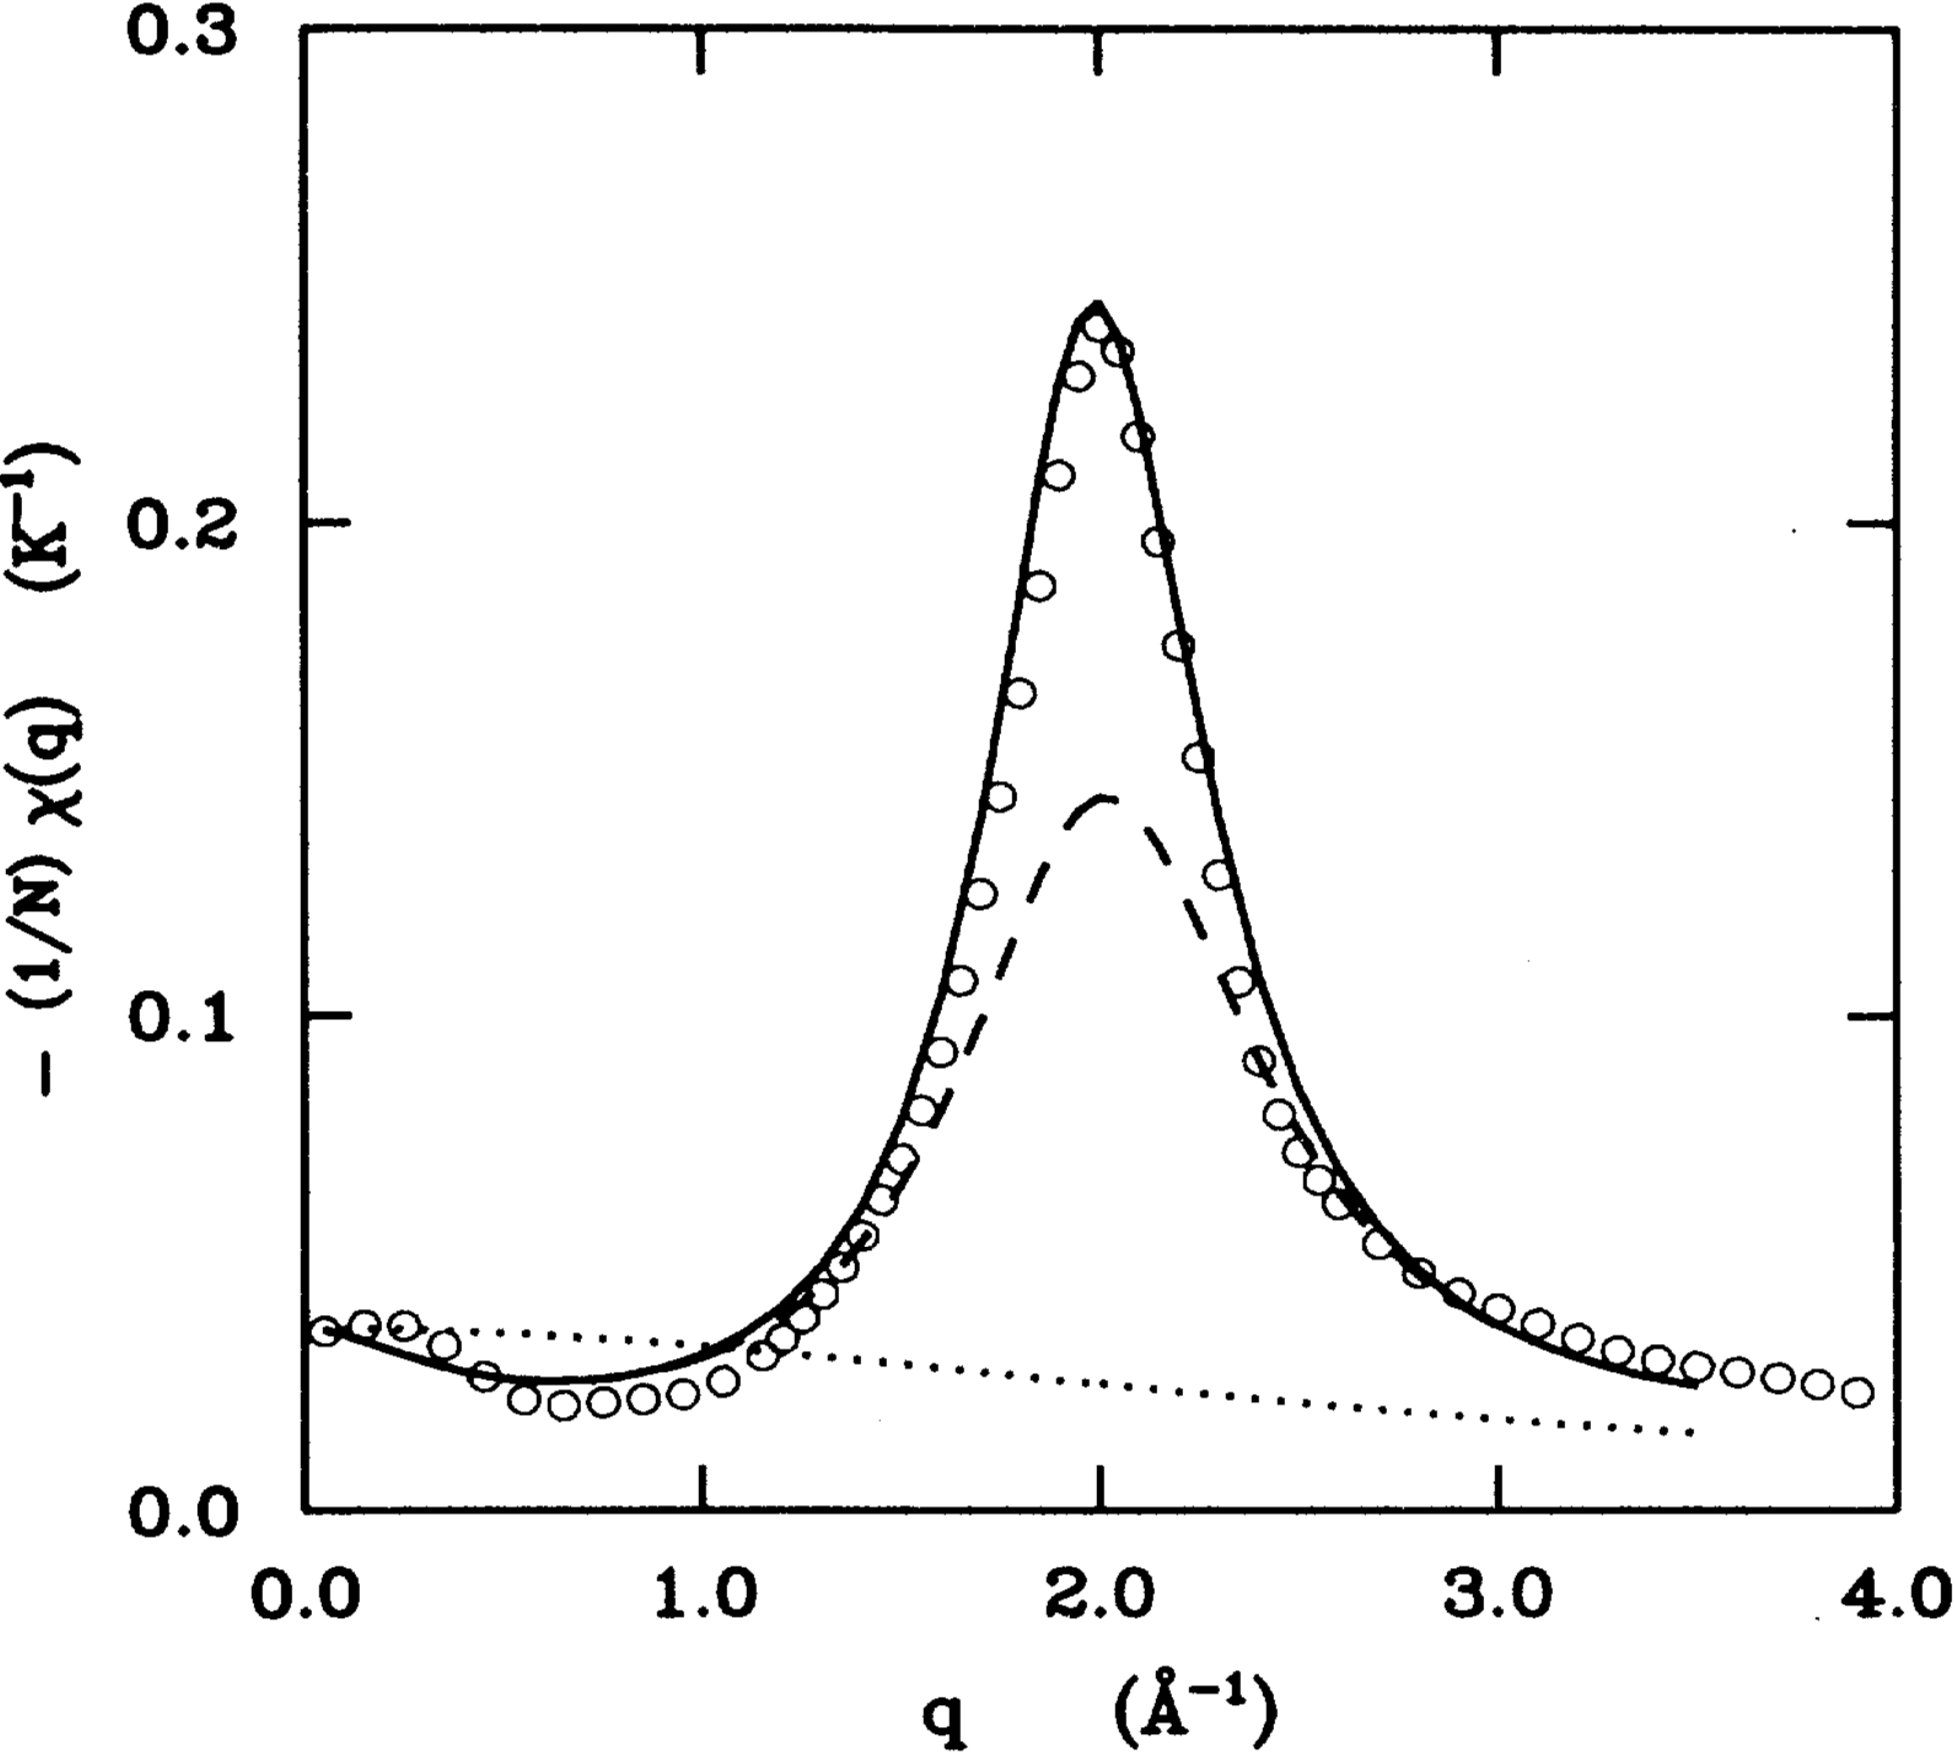
\includegraphics[width=0.75\textwidth]{static-response-function}
				\caption{Static response $-\chi$ (see\rf{Dalfovo1995}, Eqn.~(11)) per atom of liquid $^4$He at zero pressure. Points: experimental data; dotted line: from the functional of\rfs{Str87a,Str87b}; dashed line: Orsay-Paris (OP) functional\citep{Dupont-Roc1990}; solid line: OT functional.}
				\label{fig:static-response-function}
			\end{center}
		\end{figure}
	
		The functional that is used in the work presented in this thesis is based on the Orsay-Trento (OT) functional\citep{Dalfovo1995}. It uses a finite-range, non-local approach and it is, to date the most accurate model in the sense that its parameters were fitted to reproduce the bulk properties of liquid helium at $T=0=P$. It is		
		\begin{align}
			\mathcal{E}_c[\rho ,\vec{v}] &=  
			\frac{1}{2} \left.\int \! \right\{\rho({\bf r}) V_{LJ}(|{\bf r}-{\bf r'}|) \rho({\bf r'}) \nonumber \\
			&+ \left.\frac{1}{2} c_2\, \rho({\bf r}) \left[{\bar \rho}({\bf r}) \right]^2 
			+ \frac{1}{3} c_3 \, \rho({\bf r}) \left[ {\bar \rho}({\bf r}) \right]^3\right\}\diff{r'} \nonumber \\
			&- \frac{\hbar^2}{4m} \alpha_s \int \! F(|{\bf r}-{\bf r'}|) \left[ 1- \frac{{\tilde \rho}({\bf r})}{\rho_{0s}} \right]\grad{\rho({\bf r})} \cdot \grad{\rho({\bf r'})} \left[ 1- \frac{{\tilde \rho}({\bf r'})}{\rho_{0s}} \right]\diff{r'} \nonumber \\
			& - \frac{m}{4} \int \! V_J(| \mathbf{r} - \mathbf{r}'|)\, \rho(\mathbf{r}) \, \rho(\mathbf{r}')\,  [\mathbf{v}(\mathbf{r})-\mathbf{v}(\mathbf{r}')]^2\diff{r'} \label{eq:otf}
		\end{align}
		The first term corresponds to a classical Lennard-Jones type two-body interaction between helium atoms. The interaction is screened at short distances where the interaction energy is of the same order as the correlation effects:
		\begin{align}
			V_{LJ}(r) = \begin{cases}
			\epsilon_{LJ} \left[\left(\frac{\sigma}{r} \right)^{12} - \left(\frac{\sigma}{r} \right)^{6} \right] & {\rm if} \quad r > h \\
			0 & {\rm otherwise}
			\end{cases}\label{eq9}
		\end{align}
		In the second line, the terms corresponding to $c_2$ and $c_3$, correct for short range correlations when $r<h$. The weighted density $\bar{\rho}$ is the average density $\rho$ over a sphere of radius $h$:
		\begin{align}
			\bar{\rho}(\vec{r}) = \int\!\Pi_h\qty(\abs{\vec{r}-\vec{r'}})\rho({\vec{r'}})\diff{r'},
		\end{align}
		with
		\begin{align}
			\Pi_h(r) \vcentcolon= \begin{cases}
				\frac{3}{4\pi h^3} & \rm{if} \quad r\leq h \\
				0 & \rm{otherwise}
			\end{cases}
		\end{align}
		The third line is a non-local correction to the kinetic energy (KC). It partially accounts for the difference $\mathcal{T}[\rho]-T[\rho]$ mentioned in \scn{sec:kohn-sham}. The gradient-gradient interaction function $F$ is a Gaussian kernel defined as
		\begin{align}
			F(r) = \frac{1}{l^3\sqrt{\pi^3}}\unit{e}^{-r^2/l^2}
		\end{align}
		All the parameters are fitted to reproduce the peak of the static response function (see \fig{fig:static-response-function}) in the bulk liquid. The factor $\qty(1-\tilde{\rho}/\rho_{0s})$ is included to match the pressure dependence of the static response function predicted by diffusion Monte Carlo calculations\citep{Moroni1992}. The quantity $\tilde{\rho}(\vec{r})$ is another weighted density, calculated using $F$ as a weight
		\begin{align}
			\tilde{\rho}(\vec{r}) \vcentcolon= \int\!F\qty(\abs{\vec{r}-\vec{r'}})\rho(\vec{r'})\diff{r'}
		\end{align}
		The density $\tilde{\rho}(\vec{r})$ is very close to the normal density $\rho(\vec{r})$ except in very inhomogeneous situations. For helium droplets and free helium surfaces one can safely use $\rho$ instead of $\tilde{\rho}$. In the presence of significant short-range density oscillations, e.g. in the presence of heavy atomic impurities as presented in this thesis or electrons, the helium density needs to be smoothed by the Gaussian kernel $F$.  
			
		Finally, the last line in \eq{eq:otf} is called the \emph{back-flow} term and influences the dynamic response of the system. It plays the role of a non-local kinetic energy. Since the back-flow contains the factor $\vec{v}-\vec{v'}$, as defined in \eq{eq:velocity-field} the contribution will only be non-zero whenever the effective wave function $\Psi$ is complex-valued. Consequently, for time-independent case it means that this will only affect the vortex states. The phenomenological effective current-current interaction $V_J(r)$ is calibrated so that it reproduces the experimental phonon-roton spectrum (see \fig{fig:dispersion-relation}):
		\begin{align}
			V_J(r) =\,&(\gamma_{11} +\gamma_{12} \, r^2) e^{-\alpha_1 r^2} \nonumber \\
				+\,&(\gamma_{21} +\gamma_{22} \, r^2) e^{-\alpha_2 r^2}
		\end{align}
		All the parameters of the functional are given in \tab{tab:ot-params}.

		\subsection{The Solid-OT Density Functional}
			In the presence of highly inhomogeneous liquid densities, e.g. atomic impurities with a very strong He-X interaction, the OT-functional \eq{eq:otf} becomes numerically unstable. To deal with this problem an additional cut-off can be used
			\begin{align}
				\mathcal{E}^\mathrm{sol} \vcentcolon= C\rho(\vec{r})\qty{1+\tanh(\beta\qty[\rho(\vec{r})-\rho_\mathrm{m}])}
			\end{align}
			where the model parameters $\qty{C,\beta,\rho_\mathrm{m}}$ are specified in \tab{tab:ot-params}. Including this term in the OT-functional prevents excessive density build-up. $\mathcal{E}_\mathrm{sol}$ only starts to deviate from zero whenever the liquid density $\rho$ is comparable to $\rho_\mathrm{m}$ or larger. Therefore, inclusion of this term in the functional does not alter the density distribution. This penalty term was originally developed to account for the liquid-solid phase transition of $^4$He\citep{Anc05a,Cau07}. The functional that has been used to obtain the result presented in this work is refered to as the ``Solid-OT-DFT functional''. It consists of the first three terms of the original OT-functional \eq{eq:otf}, plus $E^\mathrm{sol}$
			\begin{align}
				\mathcal{E}_c^{sol}[\rho] &=  
				\frac{1}{2} \left.\int \! \right\{\rho(\vec{r}) V_{LJ}(\abs{\vec{r}-\vec{r'}}) \rho(\vec{r'}) \nonumber \\
				&+ \left.\frac{1}{2} c_2\, \rho(\vec{r}) \qty[\bar\rho(\vec{r})]^2 
				+ \frac{1}{3} c_3 \, \rho(\vec{r}) \qty[\bar\rho(\vec{r})]^3\right\}\diff{r'} \nonumber \\
				&+ C\,\rho(\vec{r})\qty\Big{1+\tanh(\beta\qty[\rho(\vec{r})-\rho_\mathrm{m}])} \label{eq:solid-otf}
			\end{align}

	\section{Static calculations}
		In the work presented here all the impurities are heavy compared to the mass of $^4$He, e.g. the mass of Rubidium is about 21 times larger than that of Helium, Xenon roughly 33 times and Argon about 10 times. Therefore we will treat the centre of mass motion of the impurities as classical. In the functional this will be modelled as an external field $V_X$, the impurity-He pair interaction
		\begin{align}
			E[\rho] \rightarrow E[\rho] + \!\int\!\rho(\vec{r})\,V_X\qty(\abs{\vec{r}-\vec{r}_I})\diff{r} \label{eq:el-static-hi}
		\end{align}
		where ${\vec r}_I$ is the location of the impurity. Varying the modified functional to minimise the energy one now finds a new EL-equation in which the helium--impurity interaction is included:
		\begin{align}
			\left\{-\frac{\hbar^2}{2m_4} \laplacian + \fdv{\mathcal{E}_c}{\rho} + V_X(|{\mathbf r} - {\mathbf r_I}|)\right\}\Psi({\mathbf r}) = \mu \Psi({\mathbf r}) \label{eq:el-static-hi}
		\end{align}
		This equation is then solved by iteration in a self-consistent way by the imaginary time propagation method\citep{Lehtovaara2007} (ITM) in cartesian coordinates. The calculations are performed in three dimensions without imposing any symmetries that are present in the external potential. All the quantities are discretised on an evenly spaced Cartesian grid with a step-size that is typically of the order of 0.4~\AA. The differential operators are evaluated using a $k$-point finite difference method where in most applications $k=13$ is sufficiently accurate. The integrals in the density-functional can be expressed as convolutions and can therefore be evaluated in momentum-space by exploiting the convolution theorem, using proprietary highly optimised parallel Fast Fourier Transform algorithms. 
			
		\subsection{Producing vortical states}\label{sec:vortical-states}
			The helium density that minimises the energy of the vortical states $\Psi_s$ (\eq{eq:line-vortex}), introduced in \scn{sec:rot-vort}, can be obtained by solving the same EL-equation as for a vortex-free droplet. This becomes clearer when we write \eq{eq:el-equation} in cylindrical coordinates:
			\begin{align}
				\qty{-\frac{\hbar^2}{2m}\qty[\frac{1}{r}\pdv{r}\qty(r\pdv{r})-\frac{s^2}{r^2}]+\fdv{\mathcal{E}_c}{\rho}}\Psi_s(\vec{r}) = \mu\Psi_s(\vec{r}) \label{eq:el-cyl}
			\end{align}
			Written like this it is evident that the ground state $\Psi_0$ is just the special case for $s=0$. Obtaining the solution using the ITM works as long as the solution has overlap with initial guess for the order parameter. Starting with a trial order parameter similar to $\Psi_s$ will guarantee this. To do this we use the ``imprinting'' technique where we use the ground state density of a previously obtained vortex-free droplet and multiply it with a normalised complex factor
			\begin{align}
				\Psi(\mathbf{r}) = \sqrt{\rho_0(\vec{r})} \,\times \frac{x + iy}{\sqrt{x^2 + y^2}} \label{eq28}
			\end{align}
			where $\rho_0$ is the ground state density of the vortex-droplet.  In cylindrical coordinates this factor is equivalent to the one in \eq{eq:line-vortex} for $s=1$. 
			
			This changes for droplets with two or more vortices, where the cylindrical symmetry is broken and the solutions are no longer solutions of \eq{eq:el-cyl}, nor eigenfunctions of the angular momentum operator. In this case the time-independent EL-equation has to be modified to include a rotational constraint solution in the co-rotating frame
			\begin{align}
				{\cal H} \rightarrow {\cal H}-\Omega \hat{L}_z
			\end{align}
			 such that for a suitable choice of $\Omega$ the vortex-array solution becomes favourable to the ground state and also to excited states with angular momentum $s\geq 2$. Since these states are no longer eigenstates of the original time-dependent Hamiltonian, these states are no longer stationary and will start to rotate with frequency $\Omega$. The initial guess for a droplet with $n_v$ vortices can be produced using the same imprinting method as mentioned before		
			\begin{align}
				\Psi(\mathbf{r})=\sqrt{\rho_0(\vec{r})} \times \prod _{j=1}^{n_v}\left[ {(x-x_j)+i(y-y_j) \over \sqrt{(x-x_j)^2+(y-y_j)^2}}  \right] \label{eq32}
			\end{align}
			where $\rho_0$ is again the ground state density of the vortex-free droplet and $(x_j,y_j)$ is the initial position of the $j$-th vortex-line parallel to the $z$-axis.

	\section{Dynamic calculations}\label{sec:td-dft}
		For the dynamic evolution of atomic impurities excited from $n$s-states to $n'$s-states, we do not need to keep track of the evolution of the electronic state of the impurity since it keeps its spherically symmetric orbital. In this case we only need to describe the time evolution of the centre of mass coordinate of the impurity. As in the statics, because of the large atomic mass of the impurity compared to helium, the time evolution of the centre of mass coordinate of the impurity is treated classically. To obtain the correct energy for the whole droplet-impurity system the energy functional needs to be extended to include the impurities centre of mass motion and the impurity-helium interaction
		\begin{align}
			E[\rho] \rightarrow E[\rho] + \frac{p^2_I}{2 m_I} + \int \! \rho(\mathbf{r}) \, V_{X^{\!*}}\qty(\abs{\vec{r}-\vec{r}_I})\diff{r} \label{eq33}
		\end{align}
		where $p_I$ is the classical momentum of the impurity, $m_I$ is the impurity mass and $V_{X^{\!*}}$ is the impurity-He pair interaction potential for an impurity in the ground-, excited $n'$s- or ionised state. The equations of motion for the time evolution of the effective wave function $\Psi\qty(\vec{r},t)$ and the second time derivative of the impurity location $\ddot{\vec{r}}_I$ are  
		\begin{align}
			i\hbar\frac{\partial}{\partial t} \Psi &= \qty[-\frac{\hbar^2}{2m_4} \laplacian +\frac{\delta {\cal E}_c}{\delta \rho} + V_{X^*}(|\mathbf{r}- \mathbf{r}_I|)]\Psi\nonumber\\
			m_I \ddot{\mathbf{r}}_I &= - \grad_{\vec{r}_I} \left[  \int \!\rho(\mathbf{r}) V_{X^*}(|\mathbf{r}- \mathbf{r}_I|)\diff{r}  \right] \nonumber \\
			&= -\int \! V_{X^*}(|\mathbf{r}- \mathbf{r}_I|)  \, \grad \rho(\mathbf{r})\diff{r} \label{eq34}
		\end{align}
	
		\subsection{The Diatomic Model}\label{sec:dim-model}
			\begin{figure}[t]
				\begin{center}
					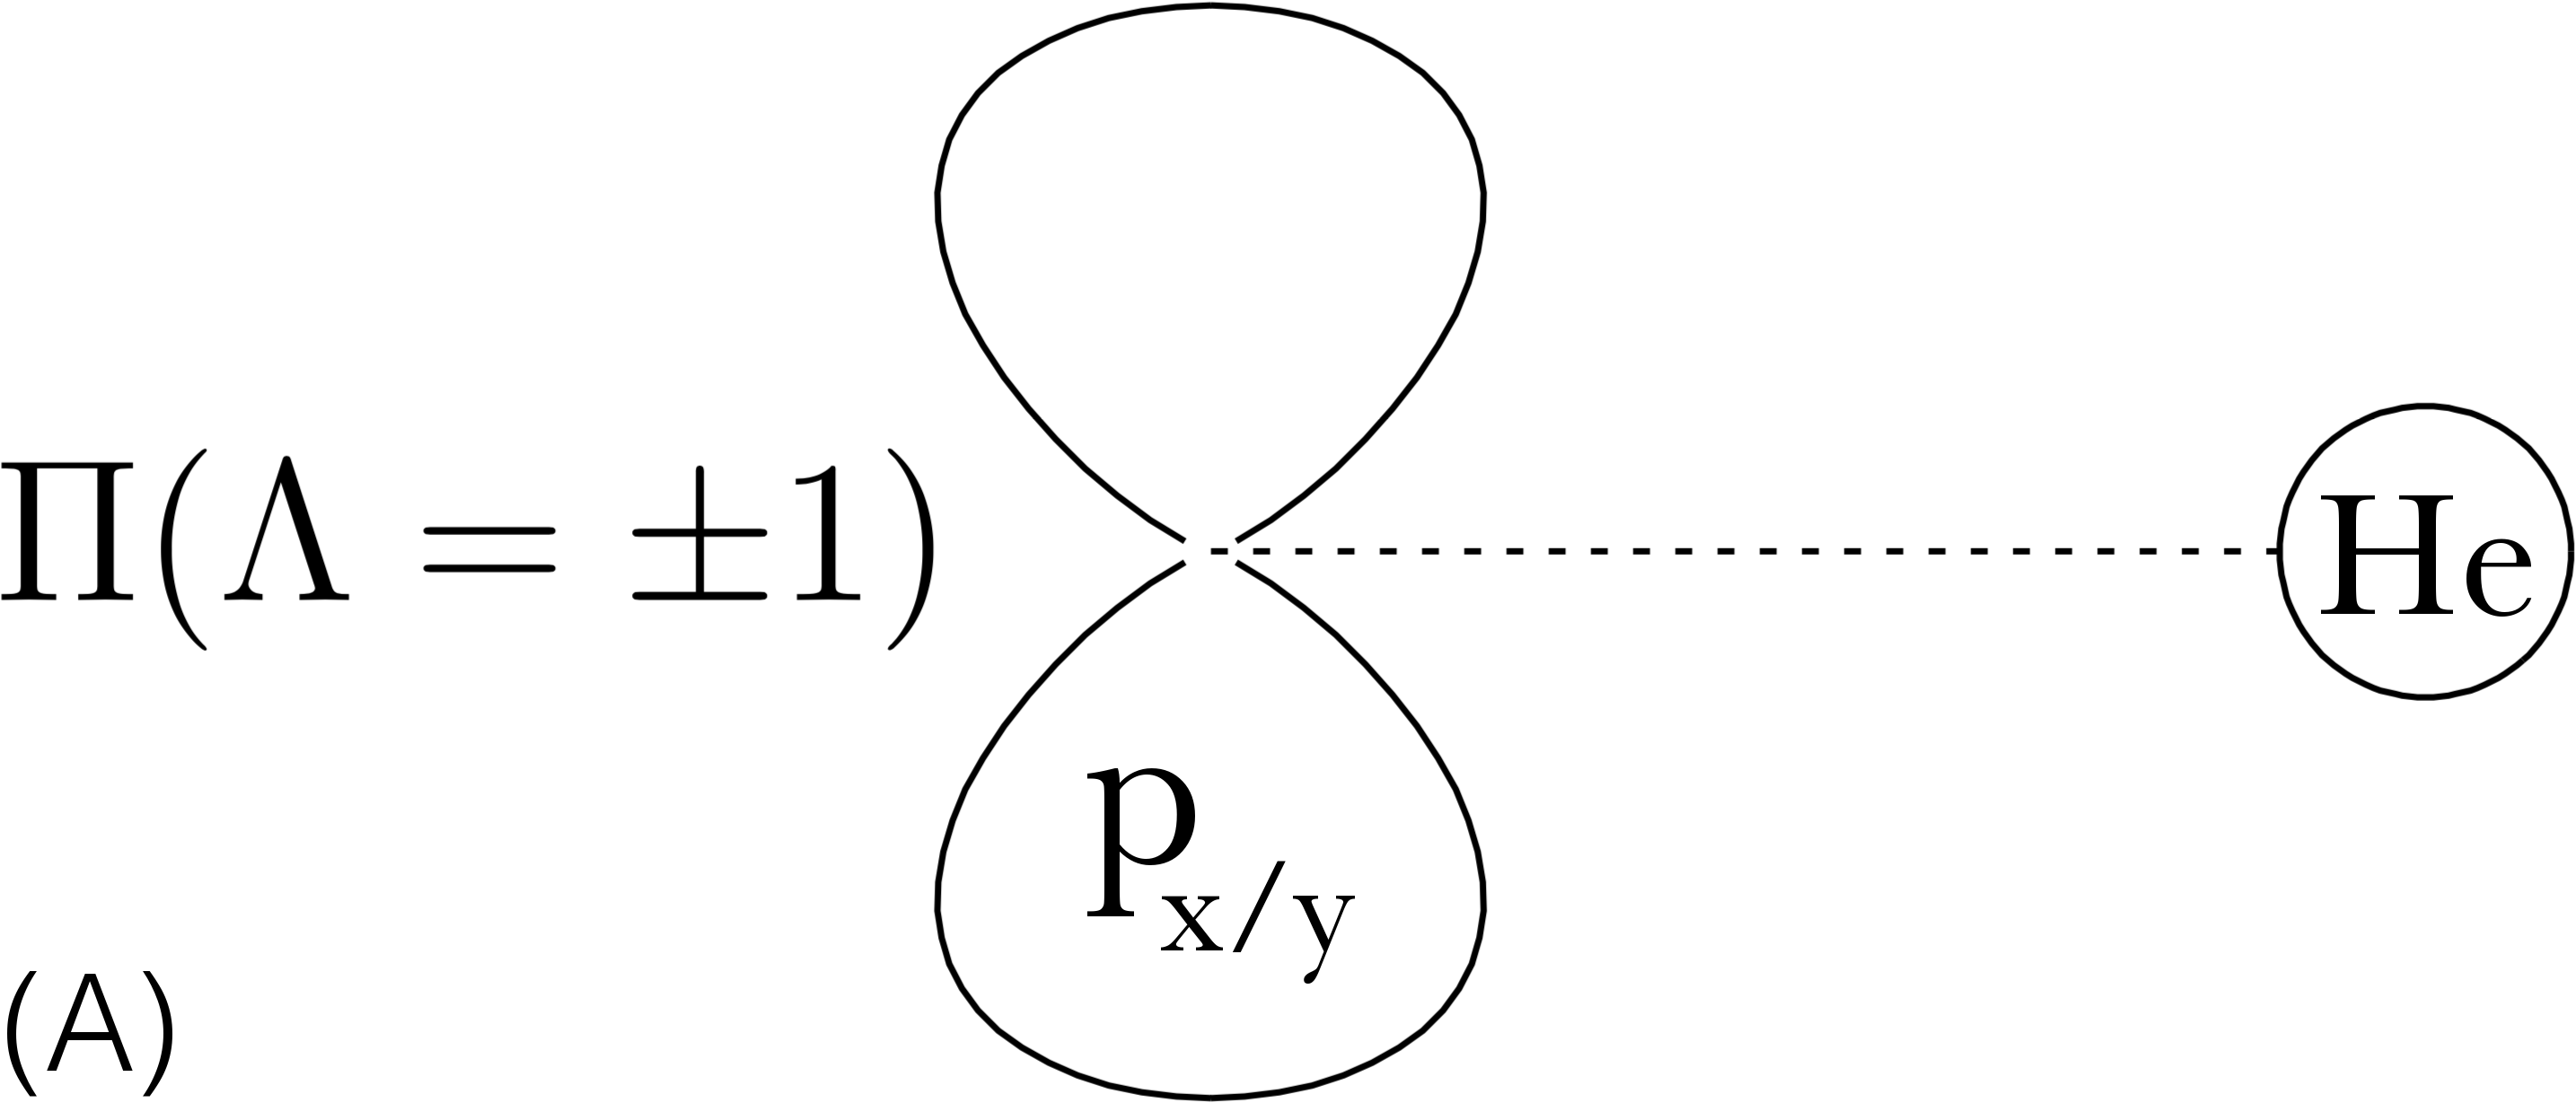
\includegraphics[width=0.45\textwidth]{pxy-he}
					\hspace{20pt}
					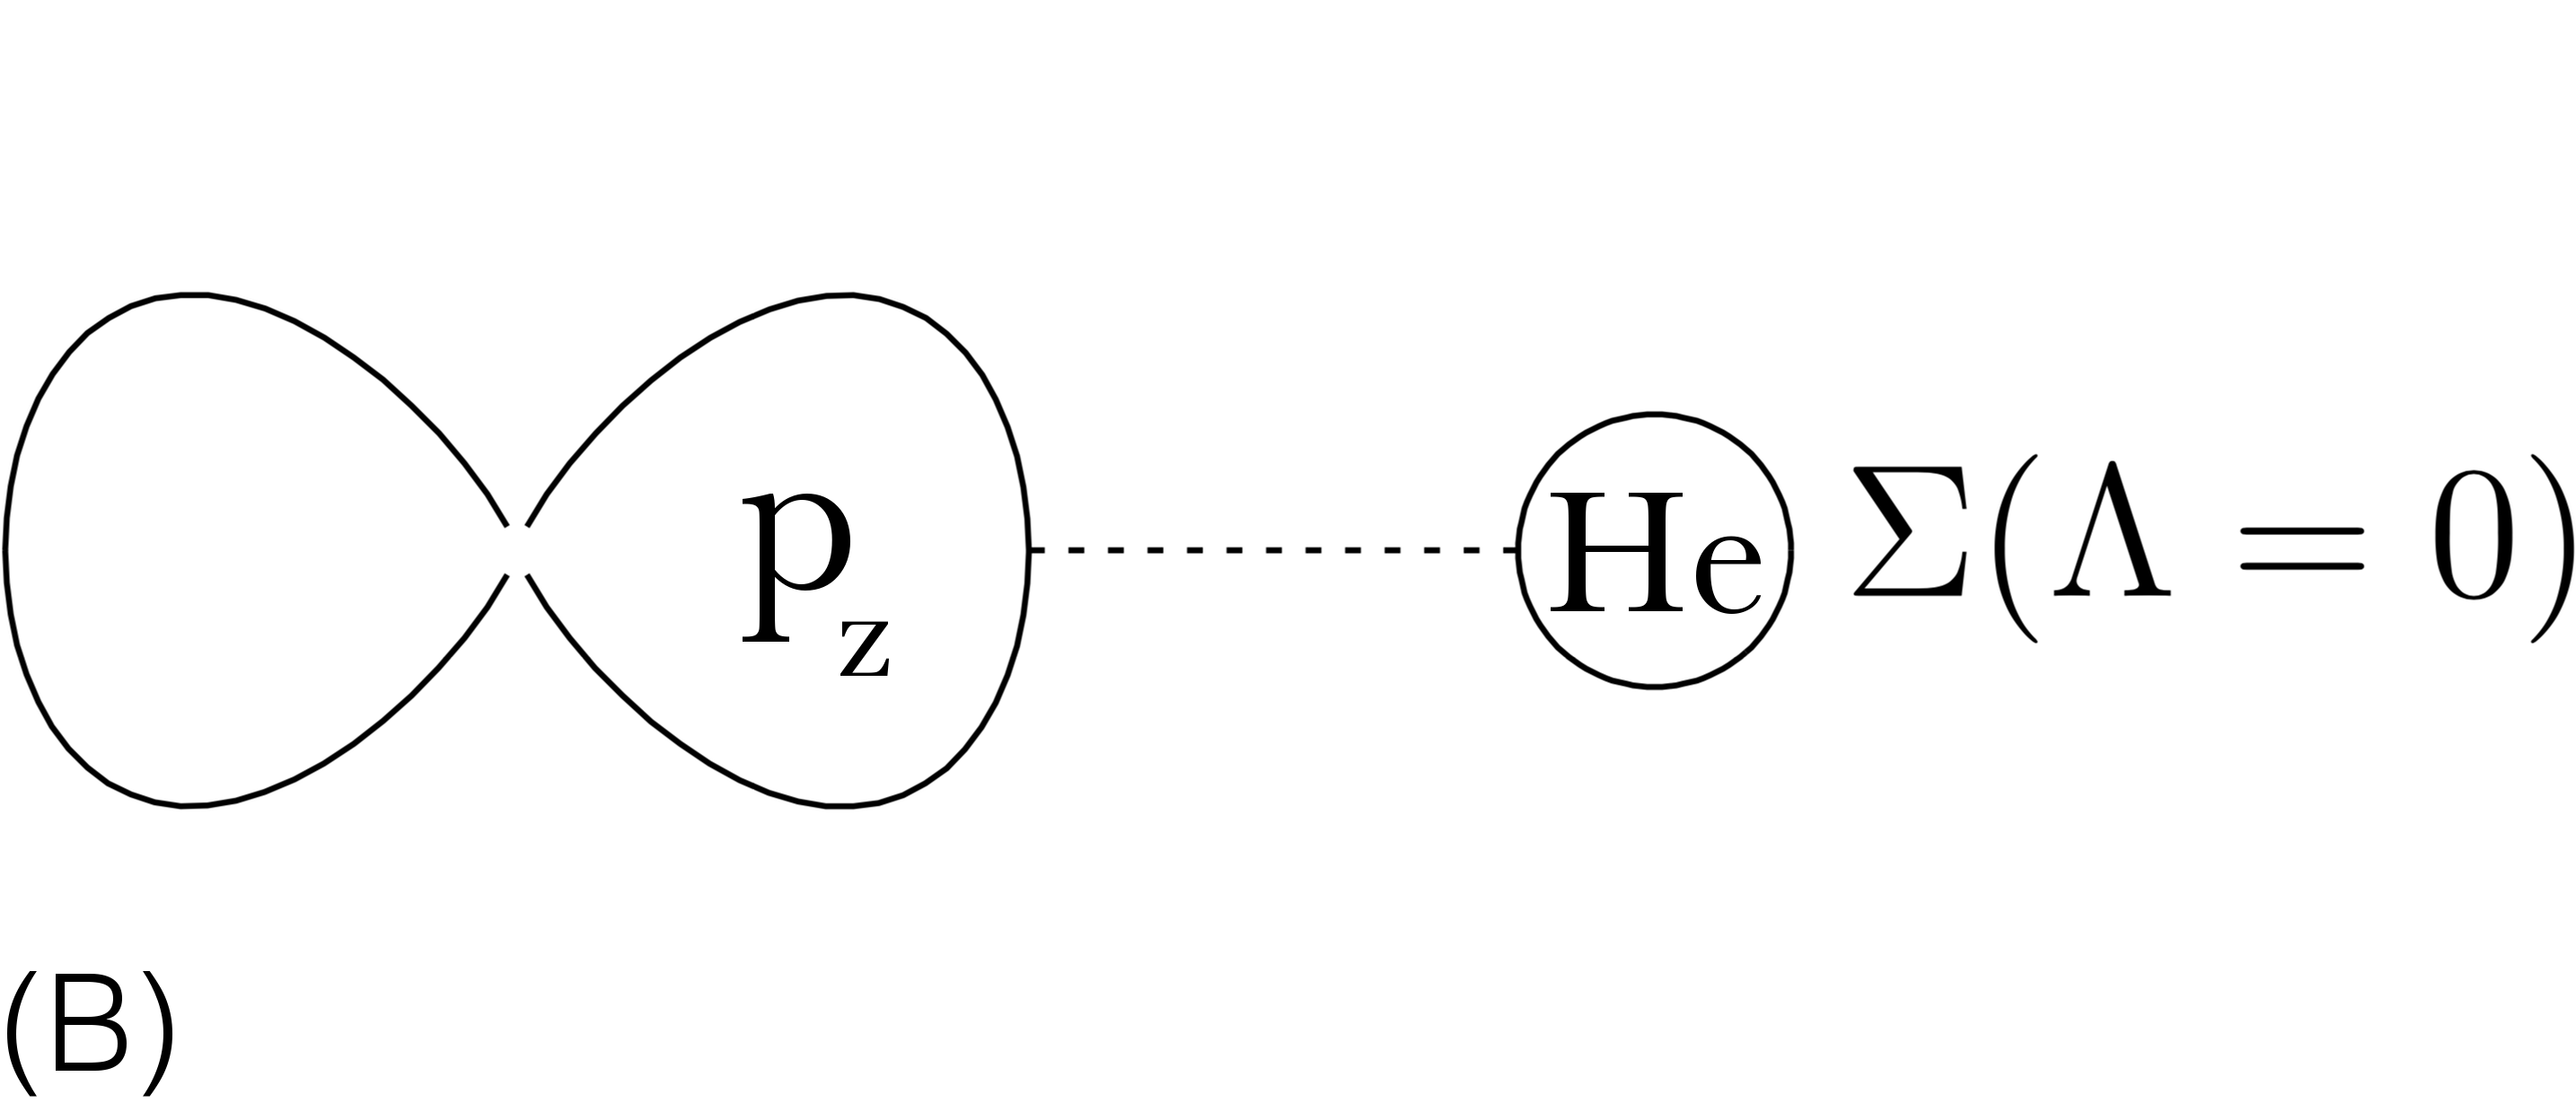
\includegraphics[width=0.45\textwidth]{pz-he}
				\end{center}
				\caption{Level splitting of the p-orbitals in the presence of helium, that breaks the spherical symmetry. (A)~A double degenerate n'p$_\mathrm{x/y}$-orbital and (B)~a single n'p$_\mathrm{z}$-orbital. (Illustration courtesy of M. Martinez\citep{Martinez2017}.)}
				\label{fig:p-orbitals}
			\end{figure}				
			The situation becomes slightly more complicated for $n$s-states excited to $n'$p-states (effective one-electron excited $^2$P-states). Since the three p-orbitals are no longer spherically symmetric and start mixing due to the interaction with the He droplet, we also need to include a description that accounts for the mixing of these orbitals in a dynamic way. To do this we use the diatomic model\citep{Ellison1963} (DIM). The interaction between a helium atom ($^1$S$_0$-state) and the triple degenerate $L=1$ electronic state of the impurity partially lifts the degeneracy so that the interaction can be decomposed into a $\Sigma$-state and a double degenerate $\Pi$-state (see \fig{fig:p-orbitals}). In the cylindrical symmetry of the DIM it is customary to use the molecular term symbol $^{2S+1}\Lambda_\Omega$ to label the levels instead of $^{2S+1}L_J$. In the bound region of the potentials $S$ is the electronic spin angular momentum (and $2S+1$ the spin multiplicity), $\Lambda$ is the modulus of the electronic orbital angular momentum and $\Omega$ is the total electronic angular momentum, all projected along the internuclear axis. Or symbolically
			\begin{align}
				\vec{J}=\vec{L}+\vec{S}\:\longrightarrow\:\vec{\Omega}=\vec{\Lambda}+\vec{S}.
			\end{align}
			 Following the spectroscopic notation the orbitals corresponding to $\Lambda=0,1,2,3,\ldots$ are labeled $\Sigma,\Pi,\Delta,\Phi,\ldots$. The interaction between a helium atom and the impurity's electronic structure can be expressed in an uncoupled basis
			\begin{align}
				 \ket{p_{im}}\in\qty\big{\,\ket{p_{xm}}\!,\ket{p_{ym}}\!,\ket{p_{zm}}} \label{eq:dim-basis}
			\end{align}
			of real one-electron p-orbitals oriented along the internuclear axis (see \fig{fig:dim-axes}). The helium-impurity interaction matrix is given by
			\begin{align}
				\mathcal{V}^{DIM}(r_m) &= V_{\Pi}(r_m)\qty\big(\dyad{p_{xm}}+\dyad{p_{ym}})+V_{\Sigma}(r_m)\dyad{p_{zm}} \nonumber \\
					&= V_{\Pi}(r_m)\qty\big(\mathbb{1}_3-\dyad{p_{zm}})+V_{\Sigma}(r_m)\dyad{p_{zm}} \nonumber \\
					&=V_{\Pi}(r_m)\mathbb{1}_3+\qty\big[V_{\Sigma}(r_m)-V_{\Pi}(r_m)]\dyad{p_{zm}}
			\end{align}	
			where $r_m$ is the modulus of the interatomic separation vector and $V_\Pi$ and $V_\Sigma$ are the $\Pi$ and $\Sigma$ impurity-He pair potentials in the absence of spin-orbit coupling. For a system consisting of $N$ helium atoms the total interaction energy is calculated by summing over all the contributions of the $N$ individual $^4$He--X contributions
			\begin{align}
				\mathcal{U}^{DIM}(\vec{r}_I)=\sum_{m=1}^{N}\mathcal{V}^{DIM}(r_m)
			\end{align}
			It is more convenient to express the interaction in a basis common to all impurity-helium pairs, instead of a basis that depends on the particular impurity-helium pair chosen. To do this we apply a rotation $\mathcal{R}_m:\hat{\vec{z}}_m\mapsto\hat{\vec{z}}\propto\vec{r}_I$, so that the matrix corresponding to the $m^{\rm th}$ $^4$He atom expressed in the common basis is given by
			\begin{align}
				\dyad{p_{zm}} = \mathcal{R}_m\dyad{p_z}\mathcal{R}_m^{-1}
			\end{align}
			It can be shown that the elements of this matrix in cartesian coordinates are of the form
			\begin{equation}
				\mel**{p_i}{\mathcal{R}_m\dyad{p_z}\mathcal{R}_m^{-1}}{p_j} = \frac{r_{im}\,r_{jm}}{\norm{\vec{r}_m}^2}		\label{eq39}
			\end{equation}	
			where $(i,j)\in\qty{x,y,z}$. With these definitions we can write the matrix elements $U^{DIM}_{ij}$ of the interaction energy $\mathcal{U}^{DIM}$
			\begin{align}
				U^{DIM}_{ij}(\vec{r}_I)=\mel**{p_i}{\mathcal{U}^{DIM}}{p_j} = \sum_{m=1}^{N} V^{DIM}_{ij}(r_m)
			\end{align}
			where
			\begin{align}
				V^{DIM}_{ij}(r_m) \vcentcolon= V_\Pi(r_m)\delta_{ij}+\qty\Big[V_\Sigma(r_m)-V_\Pi(r_m)]\frac{r_{im}\,r_{jm}}{\norm{\vec{r}_m}^2} \label{eq:vdim}
			\end{align}
			are the matrix elements of $\mathcal{V}^{DIM}$ expressed in the common basis. Since we are working with a continuous helium density $\rho(\vec{r})$ and not with discrete atoms the summation over $N$ helium atoms in the previous expression is replaced by an integral over the density $\sum_m\rightarrow\int\!\rho(\vec{r})\diff{r}$. This finally gives for the matrix element $U^{DIM}_{ij}$
			\begin{align}
				U^{DIM}_{ij}(\vec{r}_I) = \int\! \rho\qty(\vec{r}+\vec{r}_I)\,V^{DIM}_{ij}(r)\diff{r} \label{eq:u-dim}
			\end{align}
			
			The eigenvalues $U^{\mathrm{np}}_k(\vec{r}_I)$ of this real symmetric matrix define the potential energy curves (PECs) without spin-orbit coupling as a function of the distance between the surrounding helium and the impurity.
			\begin{figure}[t]
				\begin{center}
					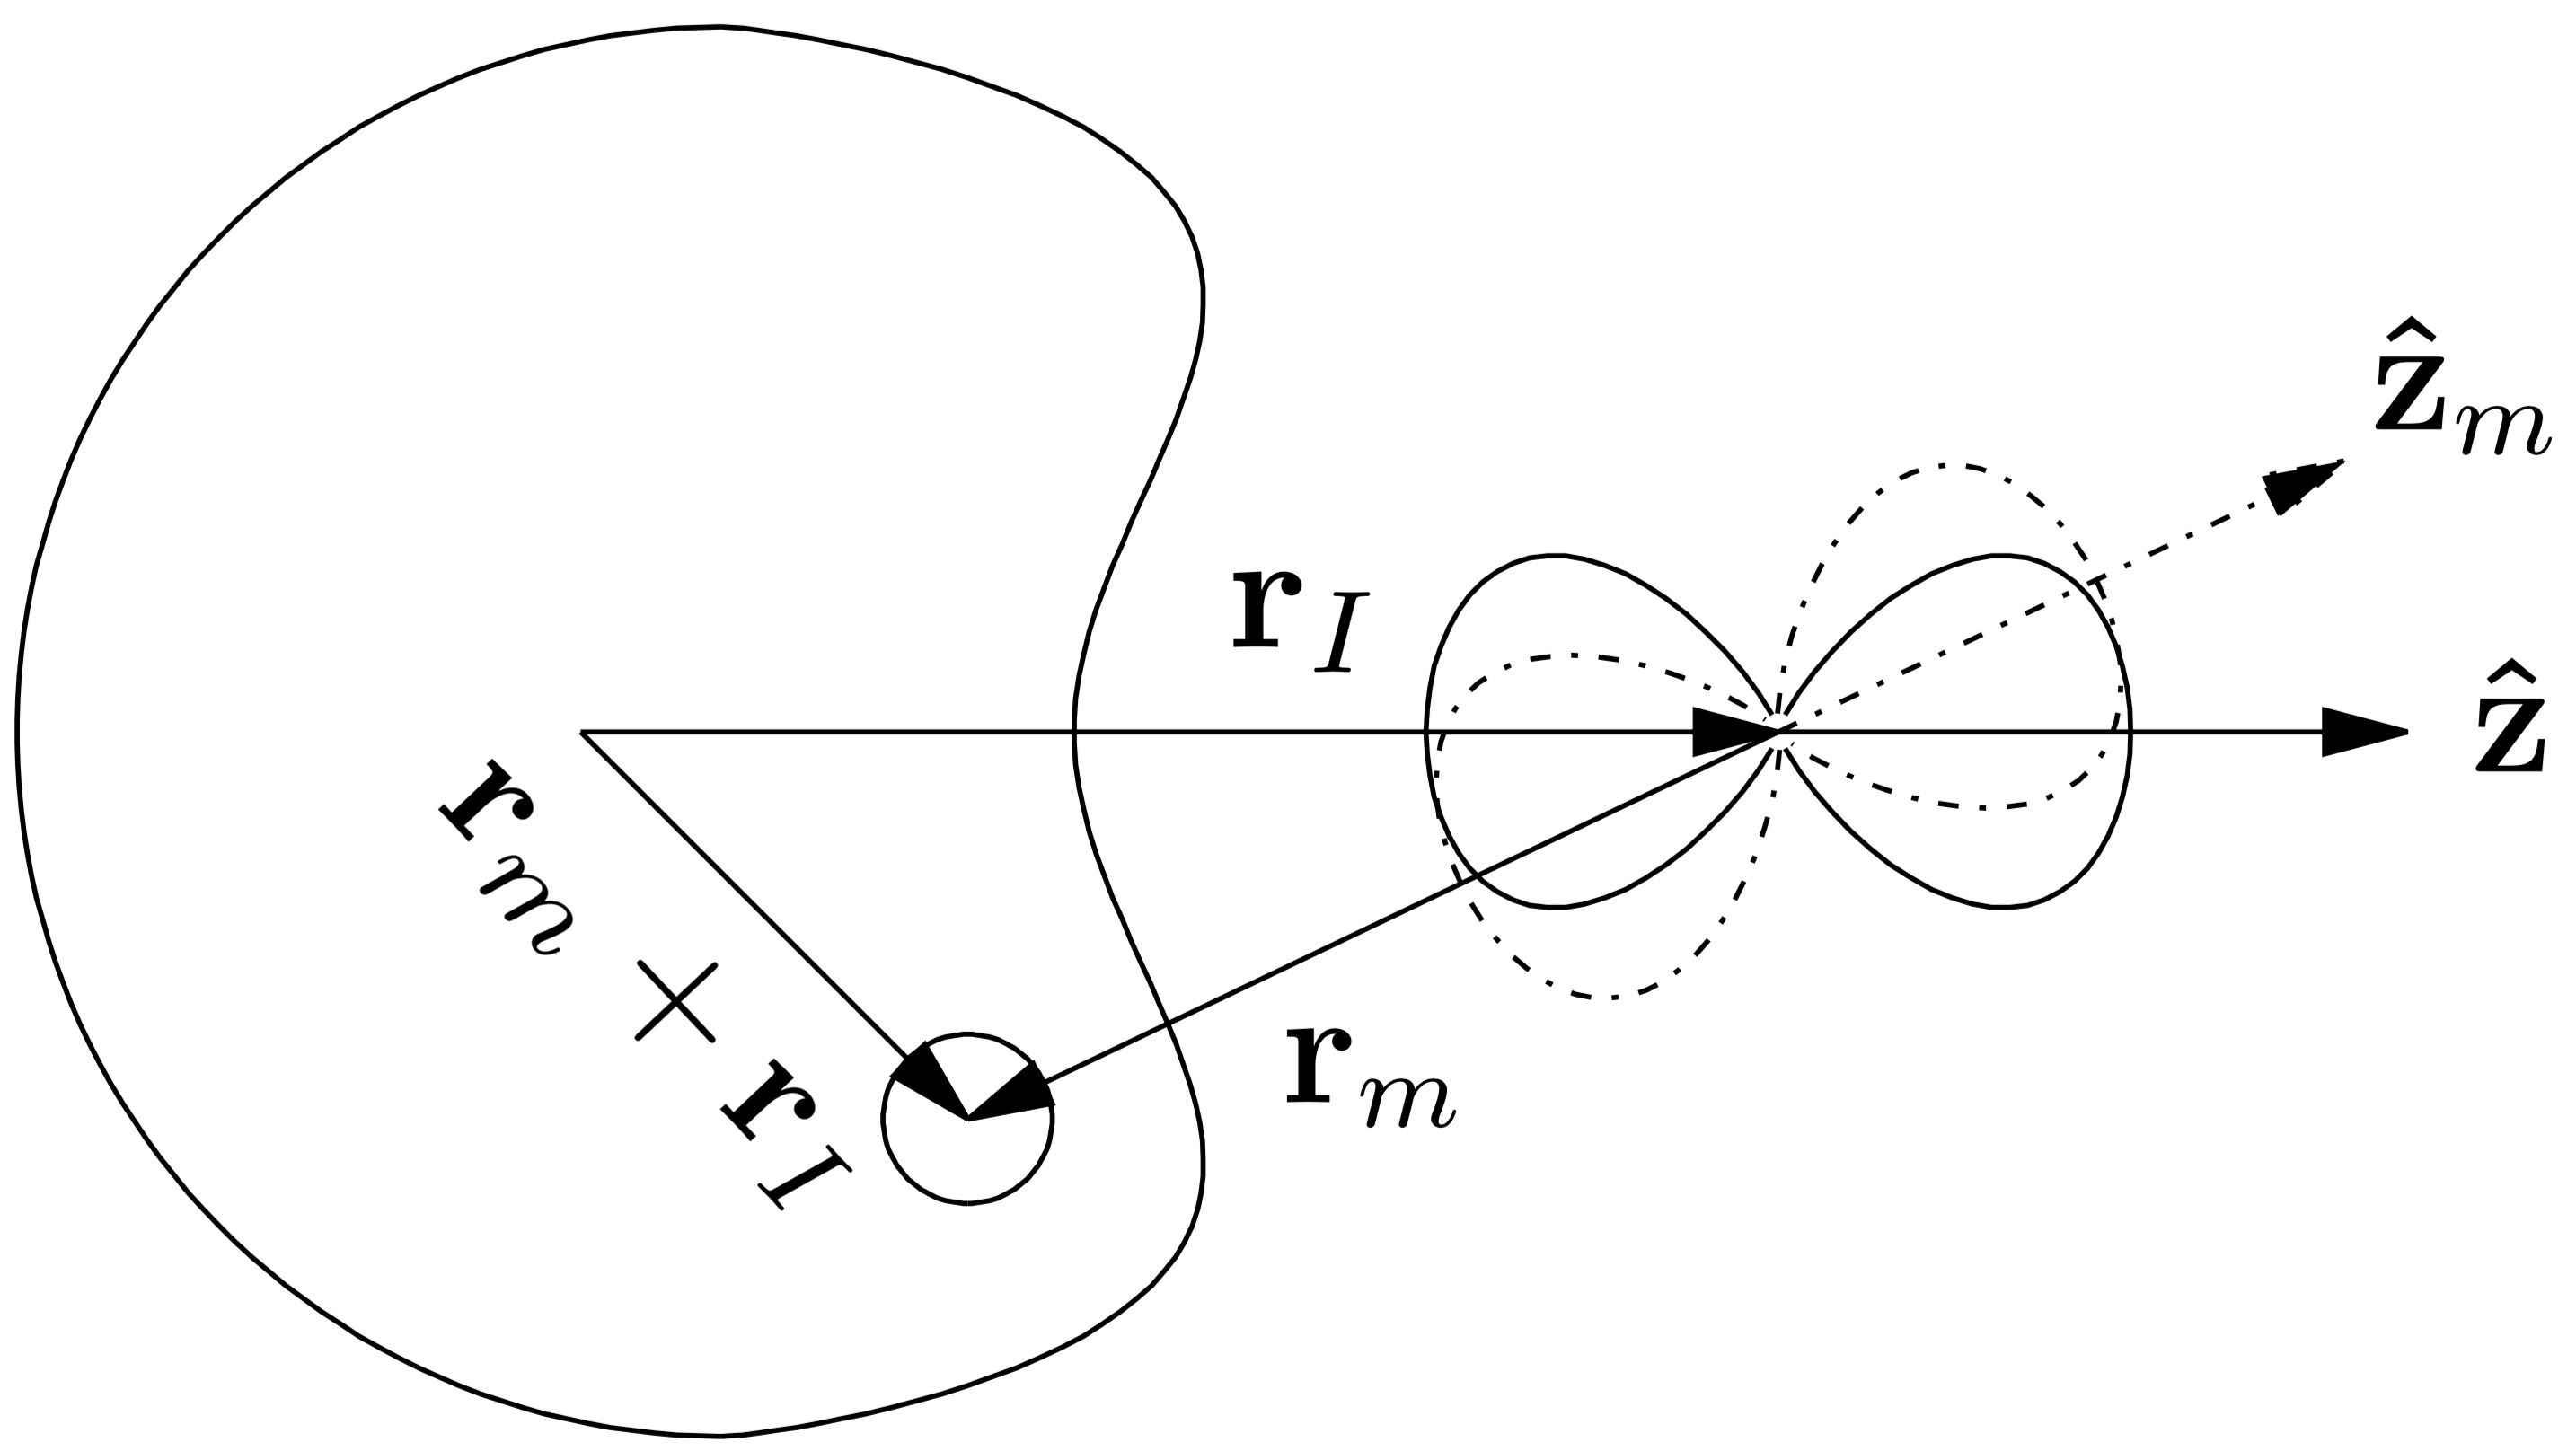
\includegraphics[width=0.75\textwidth]{dim-axes}
				\end{center}
				\caption{The set of axis defined in the DIM description. (Illustration courtesy of M. Martinez\citep{Martinez2017}.)}
				\label{fig:dim-axes}
			\end{figure}			
		
		\subsection{Including spin-orbit coupling}
			For the study of the alkali metal Rb in this work, the spin-orbit (SO) splitting of the energy levels is comparable to the splitting of the orbital angular momentum levels $\Lambda=0$ and $\Lambda=\pm 1$ due to the interaction with the helium. Therefore the spin-orbit interaction needs to be included in the total interaction Hamiltonian.
			
			The total electronic Hamiltonian is given by the sum of the DIM-interaction and the SO-interaction
			\begin{align}
				\mathcal{H} = \mathcal{U}^{DIM}+\mathcal{V}^{SO}.
			\end{align}
			The SO-matrix is approximated by the atomic alkali one, which is approximated by
			\begin{align}
				\mathcal{V}^{SO}=g\vec{L}\vdot\vec{S} = \frac{1}{2}g\qty(\vec{J}^2-\vec{L}^2-\vec{S}^2)
			\end{align}
			The coupling constant $A_{\ell s}$ is usually approximated by that of the free atom \cite{Jak97}. We can extend the DIM basis \eq{eq:dim-basis} to include the projection of the electron spin $s=\qty{\uparrow,\downarrow}$ corresponding to the quantum numbers $m_s=\qty{\frac{1}{2},-\frac{1}{2}}$:
			\begin{align}
				\ket{p_i,s}\in\qty\big{\,\ket{p_x,\uparrow}\!,\ket{p_x,\downarrow}\!,\ket{p_y,\uparrow}\!,\ket{p_y,\downarrow}\!,\ket{p_z,\uparrow}\!,\ket{p_z,\downarrow}}.
			\end{align}
			In this basis the matrix $\mathcal{V}^{SO}$ is given by
			\begin{align}
				\mathcal{V}^{SO} = \frac{1}{2}g\mqty*(0&0&-i&0&0&1\\0&0&0&i&-1&0\\i&0&0&0&0&-i\\0&-i&0&0&-i&0\\0&-1&0&i&0&0\\1&0&i&0&0&0)
			\end{align}
			Kramers' theorem states that the two-fold degeneracy of the levels originating from total half-integer spin cannot be broken by electrostatic interactions \cite{Nak01}. Therefore all the electronic eigenstates of $\mathcal{H}$ are doubly degenerate. Diagonalising $\mathcal{H}$ yields three doubly degenerate PECs between the impurity and surrounding helium.
			
			The dynamic evolution of the electronic excited state of the impurity is described by introducing an additional degree of freedom, a 6-component vector $\ket\lambda$, which describes the coefficients of the electronic state in the $\qty{\ket{p_i,s}}$ basis
			\begin{align}
				\ket{\lambda(t)} = \!\!\!\!\!\sum_{\substack{i=\{x,y,z\}\\s=\{\uparrow,\downarrow\}}}\!\!\!\!\! \lambda_{is}(t) \ket{p_i,s}
			\end{align}
			such that $\norm{\ip{\lambda}}^2=1$. The complete set of variables required to describe the
			system consists of the complex valued effective wave function for helium $\Psi(\mathbf{r}, t)$ with
			$\rho(\mathbf{r}, t) = |\Psi(\mathbf{r}, t)|^2$, the impurity position $\mathbf{r}_I(t)$, and the 6-dimensional complex vector to determine 
			its electronic wave function $|\lambda(t)\rangle$. The total energy of the impurity-$^4$He$_N$ complex after excitation to the $^2$P manifold is

			\begin{align}
				E[\Psi, \vec{r}_I, \lambda] &= \frac{\hbar^2}{2m}\int\!\abs{\grad \Psi}^2\diff{r}
				+ \int\!{\cal E}_c[\rho]\diff{r} \nonumber \\
				&+ \frac{p^2_I}{2 m_I}
				+ \int\!\rho(\vec{r})\,V_\lambda(\vec{r}-\vec{r}_I)\diff{r}
				+ \ev**{\mathcal{V}^{SO}}{\lambda}
			\end{align}
			where $V_\lambda$ is defined as
			\begin{align}
				V_\lambda(\vec{r}) \vcentcolon= \ev{\mathcal{V}^{DIM}}{\lambda} = \sum_{ijss'}\lambda^*_{is}V^{DIM}_{ijss'}(\vec{r})\lambda_{js'} 
			\end{align}
			and the components of the $6\times6$ matrix ${\mathcal V}^{DIM}$ given by
			\begin{equation}
				V^{DIM}_{ijss'}(\vec{r})=V^{DIM}_{ij}\delta_{ss'}=\qty{V_\Pi(r)\delta_{ij}+\qty\big[V_\Sigma(r)-V_\Pi(r)]\frac{r_i\,r_j}{\norm{\vec{r}_m}^2}}\delta_{ss'}
			\end{equation}
			The time evolution of the system is obtained by minimising the following action
			\begin{align}
				A[\Psi,\vec{r}_I,\lambda] = \int\!\bigg\{E[\Psi,\vec{r}_I,\lambda] -&i\hbar\int \!\Psi^*(\vec{r}) \pdv{t}\Psi(\vec{r})\dd{\vec{r}} \nonumber \\
				-&i\hbar\ev**{\pdv{t}}{\lambda} - \frac{1}{2} m_I \dot{\vec{r}}^2_I\bigg\}\dd{t} \label{eq:action}
			\end{align}
			Variation of the action $A$ with respect to $\qty\big{\Psi^*\!,\,\bra\lambda\!,\,\vec{r}_I}$ yields the following three coupled EL-equations
			\begin{align}
				i\hbar\pdv{t}\Psi &= \qty[-\frac{\hbar^2}{2m}\laplacian +\fdv{\mathcal{E}_c}{\rho(\mathbf{r})} + V_\lambda(\vec{r}-\vec{r}_I)]\Psi \nonumber \\
				i\hbar\pdv{t}\ket\lambda  &= \mathcal{H}\ket\lambda \nonumber \\
				m_I\ddot{\vec{r}}_I &= - \grad_{\vec{r}_I}\qty[\int\!\rho(\vec{r})\,V_\lambda(\vec{r}-\vec{r}_I)\dd{\vec{r}}] = -\!\int\!V_\lambda(\vec{r}-\vec{r}_I)\,\grad\rho(\vec{r})\dd{\vec{r}} \label{eq:dyn-el}
			\end{align}
			where the explicit time dependence of the variables is omitted for clarity. The second line of \eq{eq:dyn-el} is a $6\times 6$ matrix equation with the matrix elements of $\mathcal{H}$ given by
			\begin{align}
				H_{ijss'} = U^{DIM}_{ijss'}+V^{SO}_{ijss'} = \int\!\rho(\vec{r})\,V^{DIM}_{ijss'}(\vec{r}-\vec{r}_I)\dd{\vec{r}}+V^{SO}_{ijss'}
			\end{align}
			In the cases that SO-coupling can be neglected the 6-dimensional electronic state vector $\ket{\lambda}$ reduces to the 3-dimensional vector
			\begin{align}
				\ket{\lambda(t)} = \!\sum_{i=\{x,y,z\}} \!\lambda_{i}(t) \ket{p_i}
			\end{align}
			and the $6\times6$ matrix $\mathcal{H}$ reduces to the $3\times 3$ matrix of \eq{eq:u-dim} with elements
			\begin{align}
				H_{ij} = U^{DIM}_{ij} = \int\!\rho(\vec{r})\,V^{DIM}_{ij}(\vec{r}-\vec{r}_I)\dd{\vec{r}}
			\end{align}
			
			For the technical details about how this method is implemented the interested reader is directed to\rf{dft-guide}. For the collection of Fortran code that has been used to obtain the results presented here see\rf{Pi2017}. For the manuel to use the code, with included example calculations see\rf{Coppens2017}.
